\setcounter{chapCompteur}{2}
\ChapNumber{\myChapNum}{\hspace*{0.8cm}\LARGE \textbf{Fonctionnement}}{\hspace*{0.8cm}\small Des niveaux aux cases}
\section{Fonctionnement}



\begin{frame}[t,fragile]{Chaque facteur devient une liste de niveaux observés}
\vfill
{\relscale{0.9}
\texttt{\_build\_visual\_axis} retire les valeurs vides et les doublons. Si tous les niveaux d'un facteur sont numériques, ils sont triés ; sinon ils gardent leur ordre d'apparition. Les libellés sont tronqués à 36 caractères.
\begin{lstlisting}[style=py_style1,numbers=none,basicstyle=\ttfamily\footnotesize,xleftmargin=0pt,breakatwhitespace=false,breakindent=0pt,keepspaces=true,breaklines=true,linewidth=0.98\linewidth]
    unique_values = _unique_nonblank_values(values)
    if _all_numeric(unique_values):
        unique_values = sorted(unique_values, key=lambda value: float(value))
\end{lstlisting}
\begin{columns}[T,totalwidth=1.05\textwidth]
\begin{column}{0.54\textwidth}
\centering
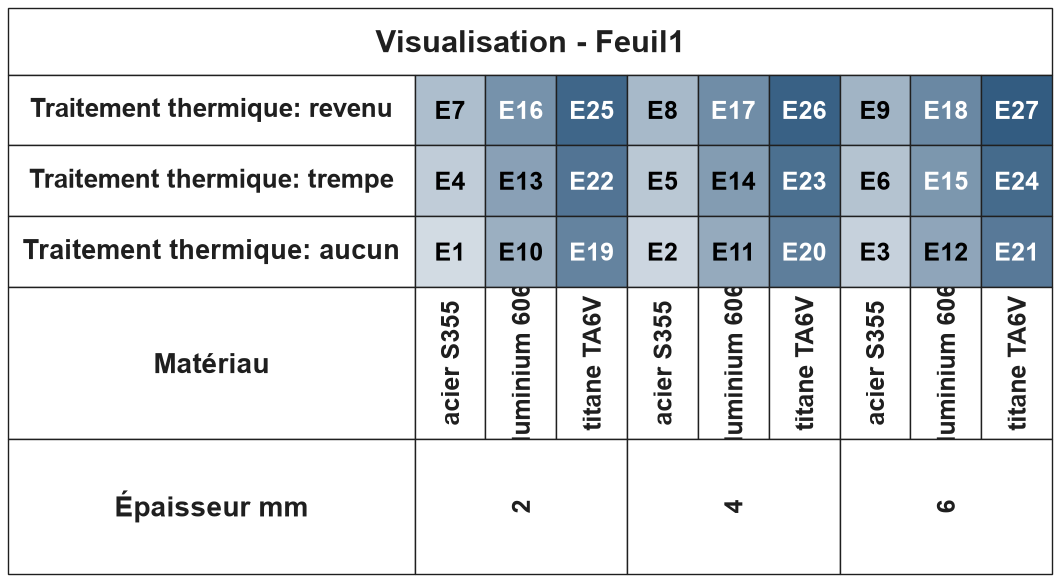
\includegraphics[width=\linewidth,height=0.34\textheight,keepaspectratio]{./_FIG/FIG_Partie_00/materiaux_textuels.png}
\end{column}
\begin{column}{0.44\textwidth}
\small Acier S355, aluminium 6061, titane TA6V : cet ordre vient du tableau. Chaque catégorie occupe une position entière. Ici toutes les cases sont remplies : c'est normal pour un plan factoriel complet ($3\times3\times3$ essais).
\end{column}
\end{columns}
\notelibre[\footnotesize]{Sortie du programme sur \texttt{materiaux\_textuels.xlsx}, données synthétiques.}}
\note{Un facteur sans aucun niveau non vide reçoit le niveau (vide).}
\vfill
\end{frame}

\begin{frame}[t,fragile]{Les pas et les indices placent chaque essai dans la grille}
% [DEVELOPPE: formule et code]
\vfill
{\relscale{0.9}
Un pas indique combien de cases franchir pour changer de niveau. \texttt{\_axis\_strides} multiplie les nombres de niveaux précédents. Les indices commencent à zéro ; le premier facteur de chaque axe varie le plus vite.
\begin{lstlisting}[style=py_style1,numbers=none,basicstyle=\ttfamily\footnotesize,xleftmargin=0pt,breakatwhitespace=false,breakindent=0pt,keepspaces=true,breaklines=true,linewidth=0.98\linewidth]
x_axes = axes[0::2]
y_axes = axes[1::2]
\end{lstlisting}
\[
s_1=1,\qquad s_j=\prod_{i<j}n_i,\qquad
x=\sum_j i_{x,j}s_{x,j},\qquad y=\sum_j i_{y,j}s_{y,j}.
\]
\begin{mybox3}[blue!5!white][Framableu][Framableu]{\textbf{Exemple L9 : pas $(1,3)$ sur chaque axe}}
x porte Vc et ap, y porte f et Lubrification. La ligne vaut $H-1-y$, avec $H=9$.\\
E1 : indices $(0,0,0,0)$, position $(x,y)=(0,0)$, ligne 8.\\
E2 : indices $(0,1,1,1)$, position $(3,4)$, ligne 4.
\end{mybox3}}
\note{Indices : Vc, f, ap, Lubrification. Sur x, Vc avance d'une case et ap de trois ; sur y, f avance d'une case et la lubrification de trois. project_fractal_2d inverse y : la ligne est comptée depuis zéro en haut. E1 est en bas à gauche. E2 : 120 m/min, 0,2 mm/tr, 1 mm, émulsion. Placement retourné (4, 3, E2, 2) ; E1 retourne (8, 0, E1, 1).}
\vfill
\end{frame}

\begin{frame}[t,fragile]{Le rang colore les cases, les collisions réunissent les essais}
% [DEVELOPPE: code, figure et piège]
\vfill
{\relscale{0.9}
Par défaut, le premier essai est clair et le dernier atteint la couleur de base. La couleur suit l'ordre des lignes, sans représenter une réponse mesurée.
\begin{lstlisting}[style=py_style1,numbers=none,basicstyle=\ttfamily\footnotesize,xleftmargin=0pt,breakatwhitespace=false,breakindent=0pt,keepspaces=true,breaklines=true,linewidth=0.98\linewidth]
def _trial_sequence_color(base_color: str, order: int, n_runs: int) -> str:
    ratio = 1.0 if n_runs <= 1 else (order - 1) / (n_runs - 1)
    return _blend_hex_colors("FFFFFF", base_color, 0.22 + (0.78 * ratio))
\end{lstlisting}
\begin{columns}[T,totalwidth=1.05\textwidth]
\begin{column}{0.54\textwidth}
\centering
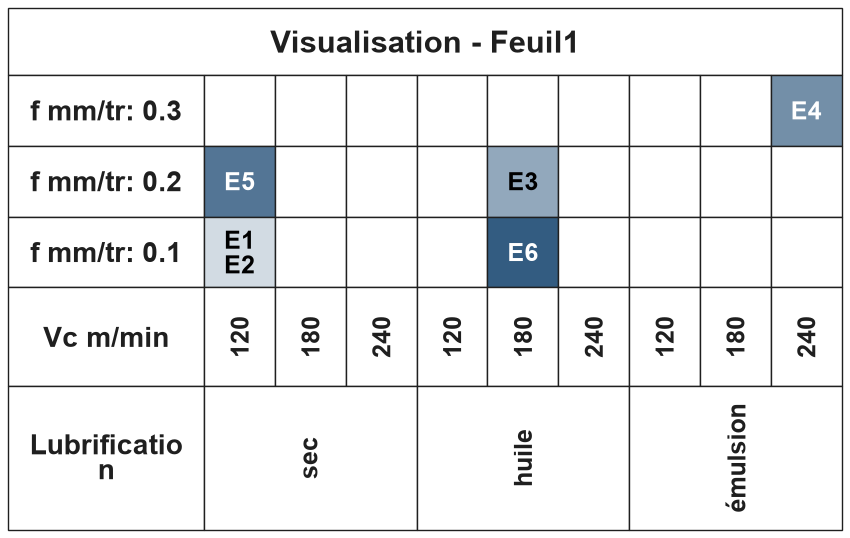
\includegraphics[width=\linewidth,height=0.34\textheight,keepaspectratio]{./_FIG/FIG_Partie_00/plan_avec_collisions.png}

{\footnotesize Données synthétiques : \texttt{plan\_avec\_collisions.xlsx}.}
\end{column}
\begin{column}{0.44\textwidth}
\raggedright
E1 et E2 partagent la même case ; sa couleur est celle du premier essai qui l'occupe. Une case blanche signale une combinaison non essayée.
\begin{mybox3}[red!5!white][Framarouge][Framarouge]{\textbf{Piège : donnée manquante}}
Vc manque pour E5 : indice zéro, ici 120, avec avertissement. Vérifier le tableau.
\end{mybox3}
\end{column}
\end{columns}}
\note{La fonction mélange du blanc à la couleur de base. Un seul essai reçoit la couleur de base. Avec neuf essais, les coefficients sont 0.22, 0.3175, 0.415, 0.5125, 0.61, 0.7075, 0.805, 0.9025 et 1. Le rang suit les lignes, même si Run n'est pas trié. Une collision garde la couleur du premier essai. Le remplissage de A1 fournit la couleur de base, sinon 335C81 ; --color l'impose. Une palette personnalisée remplace ce dégradé. Les cases blanches sont définies parmi les niveaux observés. Une donnée manquante d'un facteur utilise l'indice de niveau zéro et émet un avertissement.}
\vfill
\end{frame}

\begin{frame}[t]{Ce qu'il faut retenir}{Comment ça marche et garde-fous}
\vfill
{\relscale{0.9}
\begin{mybox3}[yellow!8!white][Framajaune][Framajaune]{\textbf{Points clés}}
\begin{itemize}\itemsep4pt
\item Les indices de niveaux et leurs pas déterminent la case.
\item La couleur suit l'ordre des lignes ; une collision réunit les identifiants.
\end{itemize}
\end{mybox3}
\begin{mybox3}[red!5!white][Framarouge][Framarouge]{\textbf{Piège : la grille croît par multiplication}}
Plafond par défaut : \numprint{90000} cases. Neuf facteurs à quatre niveaux en donnent $4^9=\numprint{262144}$. Au-delà : statut \texttt{skipped}, aucune image, message rouge dans le classeur si une sortie XLSX est demandée. Relever \texttt{-{}-max-cells} ou réduire les facteurs. \texttt{-{}-dry-run} n'écrit rien (ni classeur, ni rapport, ni image).
\end{mybox3}}
\note{Limites Excel : 16384 colonnes et 1048576 lignes, même avec --max-cells.}
\vfill
\end{frame}

\begin{frame}[plain]
\centering\vspace{1cm}
\textbf{\Huge Passer à son classeur}
\vspace{1cm}

{\large Et en pratique, comment obtenir puis vérifier cette image~?}
\end{frame}

